\title{Bayesian recurrent neural network}

\subsection{Bayesian recurrent neural network}

Random variables can also be composed with control flow operations.
As an example, we show a Bayesian recurrent
neural network (RNN) with
variable length.
The data is a sequence $\{\mathbf{x}_1,\ldots,\mathbf{x}_T\}$ of length $T$ with $D$
inputs $\mathbf{x}_t\in\mathbb{R}^{D}$ per time step.
A RNN applies the update
\begin{equation*}
\mathbf{h}_t = \text{tanh}(\mathbf{W}_h \mathbf{h}_{t-1} +
\mathbf{W}_x \mathbf{x}_t + \mathbf{b})
\end{equation*}
for $t=1,\ldots,T$, and where the previous hidden state is
$\mathbf{h}_{t-1}\in\mathbb{R}^H$.
We place a standard normal prior over its parameters
$\{\mathbf{W}_h\in\mathbb{R}^{H\times H}, \mathbf{W}_x\in\mathbb{R}^{D\times H},
\mathbf{b}\in\mathbb{R}^H\}$.

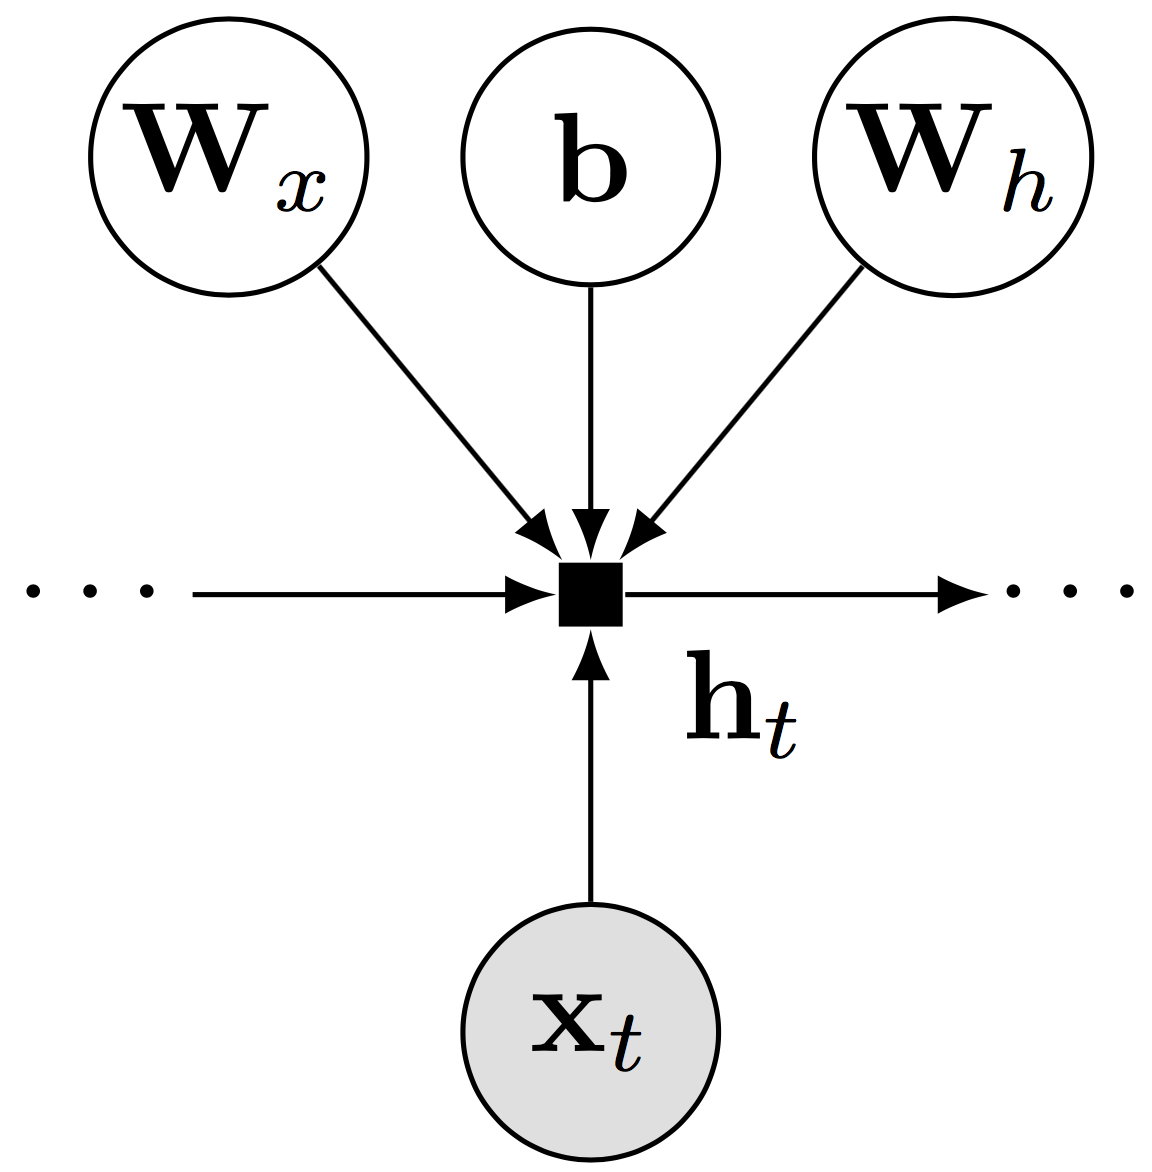
\includegraphics[width=250px]{/images/bayesian_rnn.png}

{\small\textit{Graphical model of a Bayesian recurrent neural network.}}

\begin{lstlisting}[language=python]
from edward.models import Normal

def rnn_cell(h, x):
  return tf.tanh(tf.dot(h, Wh) + tf.dot(x, Wx) + b)

Wh = Normal(mu=tf.zeros([H, H]), sigma=tf.ones([H, H]))
Wx = Normal(mu=tf.zeros([D, H]), sigma=tf.ones([D, H]))
b = Normal(mu=tf.zeros(H), sigma=tf.ones(H))

inputs = tf.placeholder(tf.float32, [None, D])
outputs = tf.scan(rnn_cell, inputs, initializer=tf.zeros(H))
\end{lstlisting}

The program has an unspecified length, leveraging a symbolic for loop
(\texttt{tf.scan}).
